\documentclass[12pt]{article}
\usepackage{latexsym,amssymb,amsmath} % for \Box, \mathbb, split, etc.
% \usepackage[]{showkeys} % shows label names
\usepackage{cite} % sorts citation numbers appropriately
\usepackage{path}
\usepackage{url}
\usepackage{verbatim}
\usepackage[pdftex]{graphicx}
\usepackage{array}
\usepackage{multirow}

% horizontal margins: 1.0 + 6.5 + 1.0 = 8.5
\setlength{\oddsidemargin}{0.0in}
\setlength{\textwidth}{6.5in}
% vertical margins: 1.0 + 9.0 + 1.0 = 11.0
\setlength{\topmargin}{0.0in}
\setlength{\headheight}{12pt}
\setlength{\headsep}{13pt}
\setlength{\textheight}{625pt}
\setlength{\footskip}{24pt}

\renewcommand{\textfraction}{0.10}
\renewcommand{\topfraction}{0.85}
\renewcommand{\bottomfraction}{0.85}
\renewcommand{\floatpagefraction}{0.90}

\makeatletter
\setlength{\arraycolsep}{2\p@} % make spaces around "=" in eqnarray smaller
\makeatother

% change equation, table, figure numbers to be counted inside a section:
\numberwithin{equation}{section}
\numberwithin{table}{section}
\numberwithin{figure}{section}

% begin of personal macros
\newcommand{\half}{{\textstyle \frac{1}{2}}}
\newcommand{\eps}{\varepsilon}
\newcommand{\myth}{\vartheta}
\newcommand{\myphi}{\varphi}

\newcommand{\IN}{\mathbb{N}}
\newcommand{\IZ}{\mathbb{Z}}
\newcommand{\IQ}{\mathbb{Q}}
\newcommand{\IR}{\mathbb{R}}
\newcommand{\IC}{\mathbb{C}}
\newcommand{\Real}[1]{\mathrm{Re}\left({#1}\right)}
\newcommand{\Imag}[1]{\mathrm{Im}\left({#1}\right)}

\newcommand{\norm}[2]{\|{#1}\|_{{}_{#2}}}
\newcommand{\abs}[1]{\left|{#1}\right|}
\newcommand{\ip}[2]{\left\langle {#1}, {#2} \right\rangle}
\newcommand{\der}[2]{\frac{\partial {#1}}{\partial {#2}}}
\newcommand{\dder}[2]{\frac{\partial^2 {#1}}{\partial {#2}^2}}
\usepackage{enumitem}
\newcommand{\nn}{\mathbf{n}}
\newcommand{\xx}{\mathbf{x}}
\newcommand{\uu}{\mathbf{u}}
\usepackage{tikz}
\usetikzlibrary{arrows}
\usetikzlibrary{positioning}
\usepackage{titlesec}
\newcommand{\junk}[1]{{}}
\usepackage{sectsty}
\usepackage{xcolor}

\newcommand\MyBox[2]{
	\fbox{\lower0.75cm
		\vbox to 1.7cm{\vfil
			\hbox to 1.7cm{\hfil\parbox{1.4cm}{#1\\#2}\hfil}
			\vfil}%
	}%
}

\makeatletter
\renewcommand*\env@matrix[1][\arraystretch]{%
	\edef\arraystretch{#1}%
	\hskip -\arraycolsep
	\let\@ifnextchar\new@ifnextchar
	\array{*\c@MaxMatrixCols c}}
\makeatother

\makeatletter
\renewcommand*\env@matrix[1][*\c@MaxMatrixCols c]{%
	\hskip -\arraycolsep
	\let\@ifnextchar\new@ifnextchar
	\array{#1}}
\makeatother

\definecolor{darkblue}{rgb}{0,0,0.4}
\usepackage[colorlinks = true,
linkcolor = darkblue,
urlcolor  = darkblue,
citecolor = darkblue,
anchorcolor = darkblue]{hyperref}
% set two lengths for the includegraphics commands used to import the plots:
\newlength{\fwtwo} \setlength{\fwtwo}{0.45\textwidth}
% end of personal macros

\begin{document}
\DeclareGraphicsExtensions{.jpg}

\begin{center}
\textsc{\Large Data Mining} \\[2pt]
	\textsc{\large Assignment 1}\\
	\vspace{0.5cm}
  Ali Gholami \\[6pt]
  Department of Computer Engineering \& Information Technology\\
  Amirkabir University of Technology  \\[6pt]
  \def\UrlFont{\em}
  \url{http://ceit.aut.ac.ir/~aligholamee}\\
    \href{mailto:aligholamee@aut.ac.ir}{\textit{aligholamee@aut.ac.ir}}
\end{center}

\begin{abstract}
In this assignment, several paramount concepts of \textit{Data Analysis} will be explained. we'll discuss the importance of metrics in the first theoretical problem. A quick review on the \textit{Apriori} algorithm for the \textit{Association Rule Mining} will be explained also. We'll also show how \textit{Weka} can be used for \textit{Association Rule Mining}. Furthermore, The effectiveness of \textit{Normalization} concept is proposed. Finally, an \textit{Statistical} point of view will help us to demonstrate and rationalize the relationship between the \textit{Performance} of the \textit{Learning Algorithm} and the amount of \textit{Data} available. A chief section of this assignment is dedicated to solve the \textit{Titanic} problem, which is a great practice of data mining concepts in production. We'll use \textit{Python} programming language and three main libraries; \textit{Scikit-Learn}, \textit{Pandas} and \textit{Numpy} to tackle this problem. The Python implementation of the Titanic problem is provided on a \textit{Jupyter Notebook} attached with this report.
\end{abstract} 

\subparagraph{Keywords.} \textit{Apriori, Association Rule Mining, Normalization, Generalization, Preprocessing, Feature Engineering, Scikit-Learn, Pandas, Numpy, Python 3.5.}

\section{Performance Metrics Analysis}
Given the following \textit{Confusion Matrix} for a prediction about cancer.

\def\arraystretch{1.5}
\begin{table}[!h]
	\centering
	\begin{tabular}{l|l|c|c|c}
		\multicolumn{2}{c}{}&\multicolumn{2}{c}{Predicted Class}&\\
		\cline{3-4}
		\multicolumn{2}{c|}{}&Cancer = Yes&Cancer = No&\multicolumn{1}{c}{Total}\\
		\cline{2-4}
		\multirow{2}{*}{Actual Class\ \ }& Cancer = Yes & $60$ & $290$ & $350$\\
		\cline{2-4}
		& Cancer = No & $150$ & $9500$ & $9650$\\
		\cline{2-4}
		\multicolumn{1}{c}{} & \multicolumn{1}{c}{Total} & \multicolumn{1}{c}{$210$} & \multicolumn{    1}{c}{$9790$} & \multicolumn{1}{c}{$10000$}\\
	\end{tabular}
	\caption{Confusion matrix of cancer prediction.}
\end{table} 
Compute each of these performance metrics.
\begin{enumerate}[label=(\alph*)]
	\item Accuracy
	\item Sensitivity
	\item Precision
	\item Specificity
	\item F-measure
\end{enumerate}

\subsection*{Solution}
Before getting into the computations, we'll review the \textit{nicknames} and \textit{formulas} to calculate each of these metrics. We have computed each of these metrics in front of them.\\
\begin{equation}
	Accuracy = \frac{TP + TN}{TP + TN + FN + FP} = \frac{60 + 9500}{60 + 9500 + 290 + 150} = 0.956
\end{equation}
\\
\begin{equation}
	TPR = Recall = Sensitivity = \frac{TP}{P} = \frac{TP}{TP + FN} = \frac{60}{60 + 290} = 0.171
\end{equation}
\\
\begin{equation}
	PPV = Precision = \frac{TP}{TP + FP} = \frac{60}{60+150} = 0.285
\end{equation}
\\
\begin{equation}
	TNR = Specificity = \frac{TN}{N} = \frac{TN}{TN + FP} = \frac{9500}{9500+150} = 0.984
\end{equation}
\\
\begin{equation}
	F-measure = \frac{2*TP}{2*TP + FP + FN} = \frac{2*60}{2*60 + 150 + 290} = 0.214
\end{equation}
Our mission is done! Nevertheless, we continue the explanation for almost each of these metrics. We'll discuss why \textit{Accuracy} itself would be a bad metric in most of the challenging cases.
\subsubsection*{Why Performance Metrics Are Important}
Metrics are important because they allow us to judge about models ability in prediction task. Without metrics we won't be able to compare models; Thus we won't be able to improve each.
\subsubsection*{What Kind of Performance Metrics Are Useful}
Not all of metrics describe this ability correctly in different conditions. Generally speaking, we need an \textit{Objective} metric. A metric could exhibit a great number for a classifier that classifies data as \textit{True} always. This can happen is \textit{Imbalanced Datasets}. The important thing is that, we need to establish a \textit{Baseline} before getting into these numbers. We need to measure the performance for a simple system before start tuning these numbers up.
The absolute maximum performance that a machine learning system can achieve, is called \textit{Ceiling}. The performance we get with respect to the numbers(\textit{like numbers calculated above}), is bound between \textit{Baseline} and \textit{Ceiling} values.
\begin{equation}
	Baseline < Performance < Ceiling
\end{equation}
\subsubsection*{Possibility of Getting Complete Performance}
No, its not possible! Even using 2 humans to classify some data, \textit{they might not agree 100\% of the times}.

\subsubsection*{Accuracy Paradox}
Accuracy is the proportion of the correct results that a classifier achieved. Assume a classifier who classifies its inputs as \textit{true} always. The denominator for the \textit{Accuracy} formula is the size of the dataset, which is a constant. The numerator while, contains $TP + TN$. This classifier predicts a great number of \textit{TP} and a small number of \textit{TN}. If the assumption changes to be that classification always turns out to be \textit{false}, we'll get a huge value for \textit{TN} and a small value for \textit{TP}. The addition is the same by the way. Thus the accuracy of a \textit{dummy} model can be amazing in both criteria. Thus, \textit{Accuracy} is not a reliable metric in machine learning problems. We call this \textit{Accuracy Paradox}. 

\subsubsection*{Recall}
This metric describes that, out of all the positive examples there were, what fraction did the classifier pick up?

\subsubsection*{Precision}
This metric states that, out of all the examples the classifier labeled as positive, what fraction were correct?

\subsubsection*{Combination of Recall \& Precision}
Combination of these metrics, causes the results to be \textit{balanced}.

\subsubsection*{$F_{\beta}$ Score}
$F_{\beta}$ combines \textit{Precision} and \textit{Recall}. We'll talk about its advantages later in this assignment.
\newpage

% Here is the association rule mining section
\section{The Association Rule Mining}
Following are four random transactions. What association rules can be found using Apriori algoirhtm?
\begin{itemize}
	\item Minimum Support: 60\%
	\item Minimum Confidence: 80\%
\end{itemize}
\begin{table}[!h] \centering
	\begin{tabular}{rcccc}
		\hline
		$ Trans\_ID $ &
		$ Item\_List $ \\
		\hline
		 T1\ \ \ \ \ & {K, A, D, B} \\
		 T2\ \ \ \ \ & {D, A, C, B, E} \\
		 T3\ \ \ \ \  & {C, A, B, E} \\
		 T4\ \ \ \ \ & {B, A, D} \\
		\hline
	\end{tabular}
	\caption{Demonstration of Database Transactions to Mine Rules From.}
	\label{tabconvdemo}
\end{table}

\subsection*{Solution}
Before getting into the details of the \textit{Apriori} algorithm, it worths mentioning that the \textit{Minimum Support} is used to find the appropriate \textit{itemset} and the \textit{Minimum Confidence} will be used to find the final \textit{rules}. Firstly, we need to find all items with size 1 and their frequencies.
\begin{table}[!h] \centering
	\begin{tabular}{rcccc}
		\hline
		$ Itemset $ &
		$ Frequency $ &
		$ Support $\\
		\hline
		 \{A\}\ \ \ \ & 4 & 100\%\\ 
		 \{B\}\ \ \ \ & 4 & 100\%\\
		 \{C\}\ \ \ \  & 2 & 50\%\\
		 \{D\}\ \ \ \ & 3 & 75\%\\
		 \{E\}\ \ \ \ & 2 & 50\%\\
		 \{K\}\ \ \ \ & 1 & 25\%\\
		\hline
	\end{tabular}
	\caption{Unity sized itemsets and their corresponding frequencies and support.}
	\label{tabconvdemo}
\end{table}
Note that in each of these sections, the value of \textit{Support} for an itemset \textit{X} can be computed using the following formula:
\begin{equation}
	Support(X) = \frac{|\{t \epsilon T;\ X 	\subseteq t\}|}{|T|}
\end{equation}
We'll continue computing the itemsets with size 2. Note that the unity sized itemsets with support less than 60\% won't be considered in this algorithm. Thus we get:
\begin{table}[!h] \centering
	\begin{tabular}{rcccc}
		\hline
		$ Itemset $ &
		$ Frequency $ &
		$ Support $\\
		\hline
		 \{AB\}\ \ \ & 4 & 100\%\\ 
		 \{AD\}\ \ \ & 3 & 75\%\\
		 \{BD\}\ \ \  & 3 & 75\%\\
		\hline
	\end{tabular}
	\caption{Itemsets of size 2 and their support.}
	\label{tabconvdemo}
\end{table}
Finally, we reach the moment that there is only 1 terminal left. The following itemset with size 3 will be the stopping point of this algorithm.
\begin{table}[!h] \centering
	\begin{tabular}{rcccc}
		\hline
		$ Itemset $ &
		$ Frequency $ &
		$ Support $\\
		\hline
		 \{ABD\}\ \ & 3 & 75\%\\ 
		\hline
	\end{tabular}
	\caption{Itemset of size 3 and its support.}
	\label{tabconvdemo}
\end{table}
We can start deriving rules from the itemset in table 2.4. To obtain the association rules, we should derive all combinations of $X \Rightarrow Y$ in this itemset. Note that in this part, we use \textit{Confidence}, which tells how often the rule found to be true. \textit{Confidence} is defined as:
\begin{equation}
	Confidence(X \Rightarrow Y) = P(Y|X) = \frac{support\_count(A \cup B)}{support\_count(A)}
\end{equation}
Thus we'll have:
\begin{itemize}
	\item $\{A,\ B\} \rightarrow \{D\} = P(D\ |\ \{A,\ B\}) = \frac{3}{3} = 1$
	\item $\{A,\ D\} \rightarrow \{B\} = P(B\ |\ \{A,\ D\}) = \frac{3}{3} = 1$
	\item $\{B,\ D\} \rightarrow \{A\} = P(A\ |\ \{B,\ D\}) = \frac{3}{4} = 0.75$
	\item $\{D\} \rightarrow \{A,\ B\} = P(\{A,\ B\ |\ \{D\}) = \frac{3}{3} = 1$
	\item $\{B\} \rightarrow \{A,\ D\} = P(\{A, D\} |\ \{B\}) = \frac{3}{3} = 1$
	\item $\{A,\ B\} \rightarrow \{D\} = P(D\ |\ \{A,\ B\}) = \frac{3}{3} = 1$
\end{itemize}
The rules with confidence above 0.8 are acceptable.
\subsubsection*{Weka Tutorial on Association Rule Mining}
In this section, we'll walk step by step to mine an association rule on an customized dataset.
\begin{enumerate}
	\item Go to the \textit{preprocess} tab. Hit the \textit{Open File} button.
	\begin{figure}[!h] \centering
		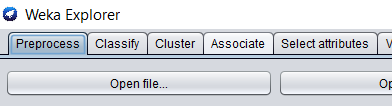
\includegraphics[width=0.5\textwidth]{openfile.png}
		\caption{Open a random dataset.}
		\label{figsolplot1}
	\end{figure}
	\item Edit the file by pressing the \textit{Edit} button.
	\begin{figure}[!h] \centering
		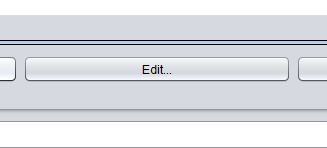
\includegraphics[width=0.5\textwidth]{edit_file.png}
		\caption{Customize the opened dataset using edit file.}
		\label{figsolplot2}
	\end{figure}

	\item Add your dataset with respect to its attributes and class values.
	\begin{figure}[!h] \centering
		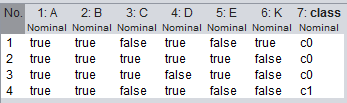
\includegraphics[width=0.5\textwidth]{data.png}
		\caption{Add samples in the database for association.}
		\label{figsolplot3}
	\end{figure}

	\item Go to the associate tab by pressing the \textit{associate} button.
	\begin{figure}[!h] \centering
		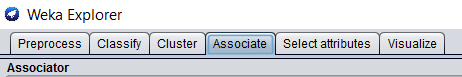
\includegraphics[width=0.5\textwidth]{associate.png}
		\caption{Open the association rules section.}
		\label{figsolplot}
	\end{figure}
	
	\item Choose the algorithm and its parameters.
	\begin{figure} \centering
		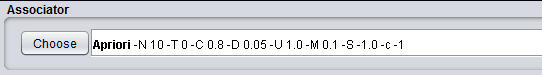
\includegraphics[width=0.5\textwidth]{select_associate_params.png}
		\caption{Tune the parameters of the algorithm.}
		\label{figsolplot}
	\end{figure}

	\item Set minimum support by filling the lower bound and upper bound support range.
	\begin{figure} \centering
		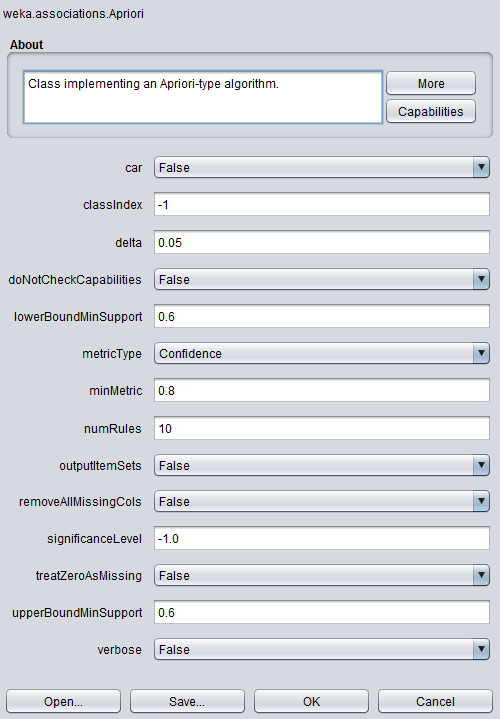
\includegraphics[width=0.5\textwidth]{set_min_support.png}
		\caption{Set the support range.}
		\label{figsolplot}
	\end{figure}
	
	\item Set the minimum confidence using the confidence form.
	\begin{figure} \centering
		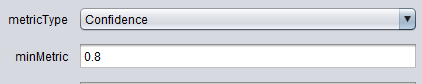
\includegraphics[width=0.5\textwidth]{set_confidence.png}
		\caption{Set the minimum confidence.}
		\label{figsolplot}
	\end{figure}
	
	\item Run the algorithm. The following is the result after hitting the \textit{start} button.
	\begin{figure} \centering
		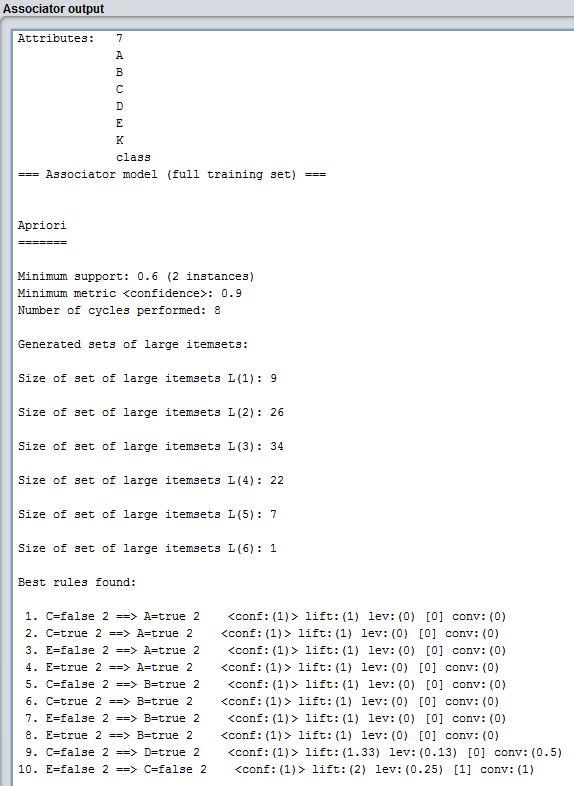
\includegraphics[width=0.6\textwidth]{associator_output.png}
		\caption{Association results.}
		\label{figsolplot}
	\end{figure}
\end{enumerate}

\newpage
\section{The Concept of Harmonic Mean and $F_{\beta}$ Score}
What is $F_{\beta}$ score? Describe how the term $\beta$ affects the final score.
\subsection*{Solution}
We saw how the $F_1$ score is computed. Before getting into the details, let's recall something interesting; \textbf{Average}.
The simplest form of average is what we describe as \textit{sum of all values divided by their count}. There is another average(\textit{mean}), which is called \textit{Harmonic mean}.\\
 Harmonic mean is represented as:
\begin{equation}
	\frac{1}{H}	= \frac{1}{n}\sum_{i=1}^{n}\frac{1}{x_{i}}
\end{equation}
Lets find the harmonic mean for two scores; Precision and Recall. The equation (2.1) turns out to be:
$$
	\frac{1}{H}	= \frac{1}{2}\sum_{i=1}^{2}\frac{1}{x_{i}}
$$	
Replacing the terms, Recall and Precision:
\begin{equation}
H = \frac{1}{\frac{1}{2}(\frac{1}{Recall} + \frac{1}{Precision})} =  \frac{2*Recall*Precision}{Recall + Precision}
\end{equation}
Generalizing this idea, we can multiply $H$ by both sides of (2.1):
\begin{equation}
	\frac{1}{n}\sum_{i=1}^{n}\frac{H}{x_i} = 1
\end{equation}

In other words, the average of ratios between the harmonic mean and the data points is unity.
We call $H$ the $F_{1}$ score. The important thing is that the effect of each score on the $H$ is considered the same here($\frac{1}{2}$). We call this effectiveness as the \textit{weight} of each score in forming the $F_{1}$ score. The summation of weights has to remain 1. Considering the the weight of $\frac{1}{\beta + 1}$ as the weight for the \textit{Precision}, we'll have $\frac{\beta}{\beta + 1}$ as the weight for the \textit{Recall}. Because we can get

$$
	\frac{\beta}{\beta + 1} + \frac{1}{\beta + 1} = \frac{\beta + 1}{\beta + 1} = 1
$$
Rewriting the equation (2.2) by changing the weights of its parameters:
\begin{equation}
	F_{\beta} = \frac{1}{\frac{\beta}{\beta + 1}\frac{1}{Recall} + \frac{1}{\beta + 1}\frac{1}{Precision}} = \frac{(\beta + 1) * Recall * Precision}{Recall + \beta*Precision}
\end{equation}
\subsubsection*{The Effect of $\beta$}
In this subsection, we'll focus on the measurements of effectiveness; \textit{Precision} and \textit{Recall}. We'll discover the \textit{effectiveness} of \textit{Precision} and \textit{Recall} on the $F_{\beta}$ score.
There are following possible conditions for the \textit{Precision} and \textit{Recall} weights.
$$
	W_{Precision} > W_{Recall}
$$
$$
	W_{Precision} < W_{Recall}
$$ 
$$ 
	W_{Precision} = W_{Recall}
$$
According to the equation (2.3), the summation of these weights is equal to 1. Thus, in order to get $ W_{Precision} = W_{Recall}$, weights are needed to be $\frac{1}{2}$ each. If $\beta > \frac{1}{2}$ the weight of \textit{Precision} is higher than the \textit{Recall} and vice versa.
In the measurement process, the users can attach different relative importance to \textit{Precision} and \textit{Recall}. What we want is therefore a parameter(\textit{$\beta$}) to characterize the measurement function in a way that \textit{It measures the effectiveness of prediction with respect to a user who attaches $\beta$ times as much importance to Recall as Precision}.

\section{The Concept of Normalization}
Describe the term \textit{Normalization} in data engineering. What do we mean by \textit{Normalizing} the data?
\subsection*{Solution}
As the word implies, \textit{Normalization} is the process of adjusting values into alignment. The \textit{transformation} of values in order to represent them in a uniform range, is also called \textit{Normalization}. This topic can have different meaning in different applications.
\subsubsection*{Normalization of Inputs in Neural Networks}
The inputs must have same range of values, otherwise we'll be left with an \textit{ill-conditioned} model after the training.

\subsubsection*{Convergence of Weights \& Biases in Distance Based Classifiers}
While using \textit{Distance Based} classifiers, it is important not to get conditioned by features with wider range of possible values. \textit{Normalization} is used to guarantee the \textit{Convergence} of \textit{Weights and Biases} in such conditions. We often call this, the \textit{Convergence of Gradient Descent}, since the gradient descent is used most of the times to optimize the loss.

\section{The Effect of Data}
  \textit{``More better data lets the model grasp a better intuition of an specific random event.''}
  This is simple expression of the \textit{Law of Large Numbers} in probability theory. The parameters of our model is tuned to predict the real-world data. It could be the data that the model has never seen while being trained. Thus, we can infer that the input data distribution will comply with the \textit{LLN} most of the times. We'll be reviewing two other effects of data in the upcoming subsections; \textit{High Variance} and \textit{High Bias} conditions.

\subsubsection*{High Variance Condition}
Occurs when a model is too complicated and relatively, the amount of data is not enough. We often call this as \textit{Overfitting} in machine learning.
The result of the criterion will be
$$
	Error_{Training} << Error_{Testing}
$$
This problem can be solved by reducing the number of features. As an example, assume a language model in which roughly every word in the vocabulary can be considered as a feature. \textit{In this case, adding more data would help}.

\subsubsection*{High Bias Condition}
Occurs when a model is too simple to explain our data. \textit{Adding more data won't help in this case.}

\end{document}